% GNUPLOT: LaTeX picture with Postscript
\begingroup
  \makeatletter
  \providecommand\color[2][]{%
    \GenericError{(gnuplot) \space\space\space\@spaces}{%
      Package color not loaded in conjunction with
      terminal option `colourtext'%
    }{See the gnuplot documentation for explanation.%
    }{Either use 'blacktext' in gnuplot or load the package
      color.sty in LaTeX.}%
    \renewcommand\color[2][]{}%
  }%
  \providecommand\includegraphics[2][]{%
    \GenericError{(gnuplot) \space\space\space\@spaces}{%
      Package graphicx or graphics not loaded%
    }{See the gnuplot documentation for explanation.%
    }{The gnuplot epslatex terminal needs graphicx.sty or graphics.sty.}%
    \renewcommand\includegraphics[2][]{}%
  }%
  \providecommand\rotatebox[2]{#2}%
  \@ifundefined{ifGPcolor}{%
    \newif\ifGPcolor
    \GPcolortrue
  }{}%
  \@ifundefined{ifGPblacktext}{%
    \newif\ifGPblacktext
    \GPblacktexttrue
  }{}%
  % define a \g@addto@macro without @ in the name:
  \let\gplgaddtomacro\g@addto@macro
  % define empty templates for all commands taking text:
  \gdef\gplbacktext{}%
  \gdef\gplfronttext{}%
  \makeatother
  \ifGPblacktext
    % no textcolor at all
    \def\colorrgb#1{}%
    \def\colorgray#1{}%
  \else
    % gray or color?
    \ifGPcolor
      \def\colorrgb#1{\color[rgb]{#1}}%
      \def\colorgray#1{\color[gray]{#1}}%
      \expandafter\def\csname LTw\endcsname{\color{white}}%
      \expandafter\def\csname LTb\endcsname{\color{black}}%
      \expandafter\def\csname LTa\endcsname{\color{black}}%
      \expandafter\def\csname LT0\endcsname{\color[rgb]{1,0,0}}%
      \expandafter\def\csname LT1\endcsname{\color[rgb]{0,1,0}}%
      \expandafter\def\csname LT2\endcsname{\color[rgb]{0,0,1}}%
      \expandafter\def\csname LT3\endcsname{\color[rgb]{1,0,1}}%
      \expandafter\def\csname LT4\endcsname{\color[rgb]{0,1,1}}%
      \expandafter\def\csname LT5\endcsname{\color[rgb]{1,1,0}}%
      \expandafter\def\csname LT6\endcsname{\color[rgb]{0,0,0}}%
      \expandafter\def\csname LT7\endcsname{\color[rgb]{1,0.3,0}}%
      \expandafter\def\csname LT8\endcsname{\color[rgb]{0.5,0.5,0.5}}%
    \else
      % gray
      \def\colorrgb#1{\color{black}}%
      \def\colorgray#1{\color[gray]{#1}}%
      \expandafter\def\csname LTw\endcsname{\color{white}}%
      \expandafter\def\csname LTb\endcsname{\color{black}}%
      \expandafter\def\csname LTa\endcsname{\color{black}}%
      \expandafter\def\csname LT0\endcsname{\color{black}}%
      \expandafter\def\csname LT1\endcsname{\color{black}}%
      \expandafter\def\csname LT2\endcsname{\color{black}}%
      \expandafter\def\csname LT3\endcsname{\color{black}}%
      \expandafter\def\csname LT4\endcsname{\color{black}}%
      \expandafter\def\csname LT5\endcsname{\color{black}}%
      \expandafter\def\csname LT6\endcsname{\color{black}}%
      \expandafter\def\csname LT7\endcsname{\color{black}}%
      \expandafter\def\csname LT8\endcsname{\color{black}}%
    \fi
  \fi
    \setlength{\unitlength}{0.0500bp}%
    \ifx\gptboxheight\undefined%
      \newlength{\gptboxheight}%
      \newlength{\gptboxwidth}%
      \newsavebox{\gptboxtext}%
    \fi%
    \setlength{\fboxrule}{0.5pt}%
    \setlength{\fboxsep}{1pt}%
\begin{picture}(9340.00,5660.00)%
    \gplgaddtomacro\gplbacktext{%
      \colorrgb{0.00,0.00,0.00}%%
      \put(752,787){\makebox(0,0)[r]{\strut{} 0,0}}%
      \colorrgb{0.00,0.00,0.00}%%
      \put(752,1252){\makebox(0,0)[r]{\strut{} 0,1}}%
      \colorrgb{0.00,0.00,0.00}%%
      \put(752,1718){\makebox(0,0)[r]{\strut{} 0,2}}%
      \colorrgb{0.00,0.00,0.00}%%
      \put(752,2183){\makebox(0,0)[r]{\strut{} 0,3}}%
      \colorrgb{0.00,0.00,0.00}%%
      \put(752,2648){\makebox(0,0)[r]{\strut{} 0,4}}%
      \colorrgb{0.00,0.00,0.00}%%
      \put(752,3114){\makebox(0,0)[r]{\strut{} 0,5}}%
      \colorrgb{0.00,0.00,0.00}%%
      \put(752,3579){\makebox(0,0)[r]{\strut{} 0,6}}%
      \colorrgb{0.00,0.00,0.00}%%
      \put(752,4044){\makebox(0,0)[r]{\strut{} 0,7}}%
      \colorrgb{0.00,0.00,0.00}%%
      \put(752,4509){\makebox(0,0)[r]{\strut{} 0,8}}%
      \colorrgb{0.00,0.00,0.00}%%
      \put(752,4975){\makebox(0,0)[r]{\strut{} 0,9}}%
      \colorrgb{0.00,0.00,0.00}%%
      \put(752,5440){\makebox(0,0)[r]{\strut{} 1,0}}%
      \colorrgb{0.00,0.00,0.00}%%
      \put(936,481){\makebox(0,0){\strut{} 0,0}}%
      \colorrgb{0.00,0.00,0.00}%%
      \put(1736,481){\makebox(0,0){\strut{} 0,1}}%
      \colorrgb{0.00,0.00,0.00}%%
      \put(2537,481){\makebox(0,0){\strut{} 0,2}}%
      \colorrgb{0.00,0.00,0.00}%%
      \put(3337,481){\makebox(0,0){\strut{} 0,3}}%
      \colorrgb{0.00,0.00,0.00}%%
      \put(4137,481){\makebox(0,0){\strut{} 0,4}}%
      \colorrgb{0.00,0.00,0.00}%%
      \put(4938,481){\makebox(0,0){\strut{} 0,5}}%
      \colorrgb{0.00,0.00,0.00}%%
      \put(5738,481){\makebox(0,0){\strut{} 0,6}}%
      \colorrgb{0.00,0.00,0.00}%%
      \put(6538,481){\makebox(0,0){\strut{} 0,7}}%
      \colorrgb{0.00,0.00,0.00}%%
      \put(7338,481){\makebox(0,0){\strut{} 0,8}}%
      \colorrgb{0.00,0.00,0.00}%%
      \put(8139,481){\makebox(0,0){\strut{} 0,9}}%
      \colorrgb{0.00,0.00,0.00}%%
      \put(8939,481){\makebox(0,0){\strut{} 1,0}}%
    }%
    \gplgaddtomacro\gplfronttext{%
      \csname LTb\endcsname%%
      \put(255,3113){\rotatebox{-270}{\makebox(0,0){\strut{}$\cos\varphi, \quad \eta$}}}%
      \csname LTb\endcsname%%
      \put(8993,3113){\rotatebox{-270}{\makebox(0,0){\strut{}}}}%
      \csname LTb\endcsname%%
      \put(4937,153){\makebox(0,0){\strut{}$P\ped{m}/P\ped{m,n}$}}%
      \csname LTb\endcsname%%
      \put(4937,5331){\makebox(0,0){\strut{}}}%
      \csname LTb\endcsname%%
      \put(4937,5440){\makebox(0,0){\strut{}}}%
      \csname LTb\endcsname%%
      \put(8289,1530){\makebox(0,0){\strut{}}}%
      \csname LTb\endcsname%%
      \put(8212,1448){\makebox(0,0)[l]{\strut{}$\cos\varphi$}}%
      \csname LTb\endcsname%%
      \put(8212,1120){\makebox(0,0)[l]{\strut{}$\eta$}}%
      \csname LTb\endcsname%%
      \put(4817,1485){\rotatebox{-270}{\makebox(0,0){$\scriptstyle\num{0,5}$}}}%
      \csname LTb\endcsname%%
      \put(1976,4789){\makebox(0,0){$\scriptstyle\num{0,8823}$}}%
      \csname LTb\endcsname%%
      \put(1976,4579){\makebox(0,0){$\scriptstyle\num{0,8000}$}}%
    }%
    \gplbacktext
    \put(0,0){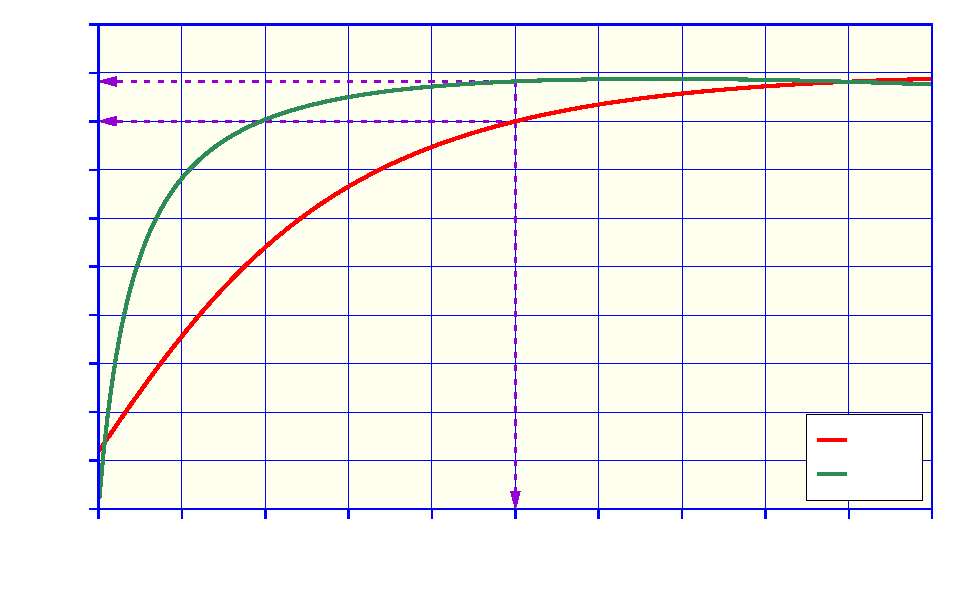
\includegraphics{Cap-Motors-Induccio-MotCarregaReduida-2}}%
    \gplfronttext
  \end{picture}%
\endgroup
